\subsection{Limiti e Continuità di funzioni in più variabili}

\subsubsection{Definizione di limiti per funzioni a più variabili}

\defn{Convergenza in \(\Rn \)}{
    Data una successione \( \{\ux_n\}\in \Rn \) questa si dice che converge a \(\ux_0 \in  \Rn \) se:

    \[
        \lim_{ n \to +\infty } d(\ux_n,\ux_0)=0
    \]

    questo equivale a dire:

    \[
        \forall \varepsilon >0 ~\exists \bar{n} \in \N \giventhat d(\ux_n,\ux_0) < \varepsilon ~\forall n \ge \bar{n}
    \]

}

\defn{Punto di accumulazione con limiti}{

    \(\ux_0\) è punto di accumulazione per \(A\) \(\iff \ux_0\) è il limite di una successione di elementi di \(A\) tutti diversi da \(\ux_0\)
}

\filbreak{}

\subsubsection*{Esempio di punti di accumulazione}

Determinare i punti di accumulazione e di frontiera dell'insieme seguente, \(A\), e stabilire se \(A\) è aperto o chiuso.

\[
    A = \{\ux \in \R^{2} \giventhat 2 < \norm{\ux} < 3 \}
\]

dove \(\ux=(x,y)\) e \(\norm{\ux} = d(\ux,\uzero) = \sqrt{x^{2}+y^{2}}\)
\begin{center}
    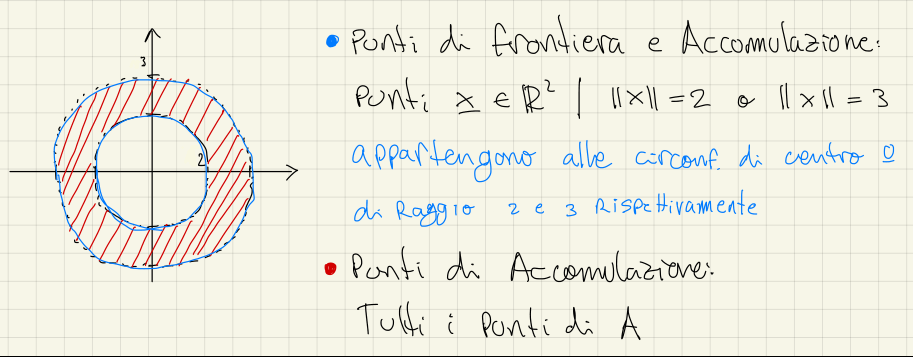
\includegraphics[width=\textwidth-2cm]{disegno-punti-di-accumulazione-esempio.png}
\end{center}

\filbreak{}

Le seguenti definizioni di limite sono equivalenti.

\defn{Limite di funzioni in più variabili con gli intorni}{
    Consideriamo ora le funzioni in più variabili
    \[f: A \subset \Rn \rightarrow \R \]
    Sia \(\ux_0 \in \Rn \) un punto di accumulazione per \(A\). Con \(l \in \R \cup \{ \pm \infty \} \), si scrive:

    \[
        \lim_{ \ux  \to \ux_0 } f(\ux ) = l
    \]

    e si dice che \(f(\ux)\) tende a \(l\) per \(\ux \) che tende a \(\ux_0\)

    se \(\forall \) intorno \(U \subset \R \) di \(l\) esiste un intorno sferico di \(\ux_0\), \(I(\ux_0,r)\) con \(r>0\),

    tale che \(f(\ux) \in U ~\forall \ux \in I(\ux_0,r) \cap \,(A \setminus \{\ux_0\})\)
}
\defn{Limite di funzioni in più variabili con epsilon-delta}{
    Consideriamo sempre le funzioni in più variabili
    \[f: A \subset \Rn \rightarrow \R \]
    Sia \(\ux_0 \in \Rn \) un punto di accumulazione per \(A\). Si scrive:

    \[
        \lim_{ \ux  \to \ux_0 } f(\ux ) = l
    \]

    e si dice che \(f(\ux)\) tende a \(l\) per \(\ux \) che tende a \(\ux_0\)

    \begin{itemize}
        \item Caso \(l \in \R \):

              se \(\forall \varepsilon>0 ~\exists \delta = \delta(\varepsilon) >0\)

              tale che \(d( f(\ux), l) < \varepsilon \quad \forall \ux \in \left( A \setminus \{\ux_0\} \right) \cap B(\ux_0, \delta)\)

              \bigskip

              Ricordando che \(d( f(\ux), l) = \norm{f(\ux) - l}\), quest'ultima condizione può anche essere scritta come:

              \ldots

              se \(\forall \varepsilon>0 ~\exists \delta = \delta(\varepsilon) >0\)

              tale che \(\norm{f(\ux) - l} < \varepsilon \quad \forall \ux \in A \setminus \{\ux_0\} \giventhat \norm{\ux - \ux_0} < \delta \)

        \item Caso \(l = +\infty \):

              se \(\forall M>0 ~\exists \delta >0\)

              tale che \(f(\ux) > M \quad \forall \ux \in A \setminus \{\ux_0\} \giventhat \norm{\ux - \ux_0} < \delta \)

    \end{itemize}

}

\filbreak{}

\subsubsection{Proprietà dei limiti di funzioni in più variabili}

Adesso parliamo di un po' di proprietà:

\begin{itemize}
    \item Il limite quando esiste è \textbf{unico}
    \item I limiti di \textbf{somme} e di \textbf{prodotti} di funzioni sono dati dalla somma e dal prodotto dei limiti (qualora i limiti esistano e le operazioni siano ben definite)
    \item Il limite del \textbf{quoziente} di due funzioni è il quoziente dei limiti (se definito)
\end{itemize}

\proposizione{}{
    Sia \(f: A \subset \R^2 \to \R \);

    Sia \(P_0=(x_0,y_0)\) punto di accumulazione per \(A\);

    Se vale:

    \[
        \lim_{ (x,y) \to (x_0,y_0) } f(x,y)=l
    \]

    allora, per ogni sottoinsieme \(C\) di \(A\) dove \(P_0\) è un punto di accumulazione per \(C\), deve valere:

    \[
        \lim_{\begin{smallmatrix} (x,y) \to (x_0,y_0) \\ (x,y) \in C \end{smallmatrix}} f(x,y)=l
    \]
}

\pagebreak

\subsubsection{Esempi di esercizi}

Abbiamo due tipologie di esercizi:

\begin{enumerate}
    \item Ci viene chiesto di analizzare cosa fa la funzione quando tende a un punto di accumulazione.

          In questo caso possiamo applicare la definizione di limite per arrivare a capire cosa succede.
    \item Ci viene chiesto di dimostrare che il limite non esiste.

          In questa tipologia di esercizi abbiamo un limite che non esiste e dobbiamo dimostrare che questa cosa è vera. Per far ciò, bisogna studiare la funzione lungo delle curve apposite lungo le quali il limite tende a valori diversi. Avendo trovato due limiti diversi, possiamo quindi concludere che non esiste per la proprietà di unicità dei limiti.

          Queste curve lungo cui studiare la funzione vanno proposte in base al tipo di funzione che abbiamo. Non c'è una regola generale per trovarle.
\end{enumerate}

\subsubsection*{Esempio 1}

Sia
\[
    f(x,y) = \frac{x^{2}}{\sqrt{x^{2}+y^{2}}}
\]

dove il dominio è \(f: \underbrace{\R^{2}\setminus \{(0,0)\}}_\text{A aperto}\rightarrow \R \)

Il punto \((0,0)\) è punto di accumulazione per \(A\)

Vogliamo vedere che succede quando la funzione tende a questo punto di accumulazione. Dimostriamo che:

\[
    \lim_{ (x,y) \to (0,0) } f(x,y) = 0
\]

ovvero che \(\forall \varepsilon >0 ~\exists \delta >0\) tale che \(|f(x,y) -0| < \varepsilon \) \(\forall (x,y) \in A\) con \(0< \sqrt{x^{2}+y^{2}}<\delta \).

Quindi \(~\forall (x,y) \in A\)

\[
    0 \le f(x,y) = \frac{x^{2}}{\sqrt{x^{2}+y^{2}}} \le \frac{x^{2}+y^{2}}{\sqrt{x^{2}+y^{2}}} \overset{\text{razionalizzo}}{=} \sqrt{x^{2}+y^{2}}
\]

E dunque  \(\forall \varepsilon > 0\) si ha:

\[
    0 \le f(x,y) < \varepsilon \qquad \forall (x,y) \neq (0,0) \giventhat[\Big] \sqrt{x^{2}+y^{2}} < \varepsilon
\]

\filbreak{}
\subsubsection*{Esercizio per casa}

Mostrare che il seguente limite non esiste:

\[
    \lim_{ (x,y) \to (0,0) } \frac{x}{\sqrt{x^{2}+y^{2}}}
\]

Se calcolo la funzione in \(y=0\):

\[
    f(x,0) = \frac{x}{\sqrt{x^{2}}}= \frac{x}{|x|}
\]

questa fa:

\begin{equation*}
    \begin{cases}
        1  & x > 0 \\
        -1 & x < 0
    \end{cases}
\end{equation*}

Il limite quindi non esiste perché ha valori diversi a seconda del caso, mentre dovrebbe essere unico, quindi concludo che non esiste.

\filbreak{}
\subsubsection*{Esercizio 1}

Mostriamo che non esiste il seguente limite:

\[
    \lim_{ (x,y) \to (0,0) } \frac{xy}{x^{2}+y^{2}}
\]

\[
    f: \R^2 \setminus \{(0,0)\} \to \R
\]

Facciamo restrizione lungo l'asse x (\(y=0\)):

\[
    C = \{(x,y) \in \R^2 \giventhat x \neq 0 \land y = 0\}
\]

Su \(C\), \(f(x,0) = 0\), infatti:

\[
    \lim_{\begin{smallmatrix} (x,y) \to (0,0) \\ (x,y) \in C \\ y=0 \end{smallmatrix}} f(x,y) = \lim_{x \to 0} f(x, 0) = 0
\]

Facciamo restrizione lungo l'asse y (\(x=0\)):

\[
    C = \{(x,y) \in \R^2 \giventhat x = 0 \land y \neq 0\}
\]

Su \(C\), \(f(0, y) = 0\), infatti:

\[
    \lim_{\begin{smallmatrix} (x,y) \to (0,0) \\ (x,y) \in C \\ x=0 \end{smallmatrix}} f(x,y) = \lim_{y \to 0} f(0, y)  = 0
\]

Proviamo a studiare la funzione lungo la bisettrice del primo e del terzo quadrante \(y=x\):

\begin{align*}
    \lim_{\begin{smallmatrix} (x,y) \to (0,0) \\ y=x \end{smallmatrix}} f(x,y) & = \lim_{ x \to 0 } f(x,x)                    \\
                                                                               & = \lim_{ x \to 0 } \frac{x^{2}}{x^{2}+x^{2}}
    = \lim_{ x \to 0 } \frac{x^{2}}{2x^{2}}
    = \frac{1}{2}
\end{align*}

Dunque, il limite non esiste.

\filbreak{}
\subsubsection*{Esercizio 2}

Dimostrare che il seguente limite non esiste

\[
    \lim_{ (x,y) \to (0,0) } \frac{3xy^{2}}{x^{2}+y^{4}}
\]

\(f:\R^{2}\setminus (0,0) \rightarrow \R \)

Lungo l'asse \(x\), ovvero per \(y=0\), il limite viene 0; anche lungo l'asse \(y\), ovvero per \(x=0\), il limite viene 0.

Provo quindi considerando tutte le rette (fascio di rette) passanti per l'origine:

\[
    y= mx
\]

con \(m \neq 0\) e \(x \neq 0\):

\begin{align*}
    \lim_{\begin{smallmatrix} (x,y) \to (0,0) \\ y=mx \end{smallmatrix}} f(x,y) & = \lim_{ x \to 0 } f(x,mx)                                                                  \\
                                                                                & = \lim_{ x \to 0 } \frac{3m^2x^3}{x^2+m^4x^4} = \lim_{ x \to 0 } \frac{3m^2x}{1+m^4x^2} = 0
\end{align*}

Provo allora lungo una parabola \(y^{2}=x\):

\begin{align*}
    \lim_{\begin{smallmatrix} (x,y) \to (0,0) \\ x=y^{2} \end{smallmatrix}} f(x,y) & = \lim_{ y \to 0 } f(y^{2},y)                                                                                    \\
                                                                                   & = \lim_{ y \to 0 } \frac{3y^{4}}{y^{4}+y^{4}} = \lim_{ y \to 0 } \frac{3y^{4}}{2y^{4}}      = \frac{3}{2} \neq 0
\end{align*}

Dunque, il limite non esiste.

\pagebreak

\subsubsection{Definizione di continuità per funzioni in più variabili}

\defn{Continuità}{
    Sia \(f: A \subseteq \R^2 \to \R \) una funzione e sia \(P_0 = (x_0, y_0) \in A\) un punto di accumulazione per A.

    Si dice che la funzione \(f\) è continua in \(P_0\) se:

    \[
        \lim_{ (x,y) \to (x_0, y_0) } f(x,y) = f(x_0, y_0)
    \]

    \begin{itemize}
        \item Se \(P_0\) è un punto isolato per \(A\), per convenzione, \(f\) è continua in tal punto.
        \item \(f\) è continua in \(A\) se è continua in tutti i punti di \(A\)
    \end{itemize}
}

Questa definizione è generalizzabile per \(\Rn \)

\subsubsection*{Esempi}

Avendo queste due funzioni

\[
    f(x,y) = x \qquad f: \R^2 \to \R
\]
\[
    g(x,y) = y \qquad g: \R^2 \to \R
\]

devo far vedere che \(f\) e \(g\) sono continue in ogni punto \(P_0 = (x_0,y_0) \in \R^2 \):

\textbf{Consideriamo la \(f\)}:

Sia dunque \(\varepsilon >0\) dobbiamo mostrare che

\[
    \exists \delta= \delta(\varepsilon) >0 \giventhat d(f(x,y)- f(x_0,y_0)) < \varepsilon \text{ se } d(P,P_0) < \delta
\]

Allora, possiamo dire che:

\[
    d(P,P_0) = \sqrt{{(x-x_0)}^{2}+{(y-y_0)}^{2}}
\]
inoltre, anche:
\[
    d(f(x,y)- f(x_0,y_0)) = |x-x_0|
\]

Mostriamo quindi:

\[
    \sqrt{{(x-x_0)}^{2}+{(y-y_0)}^{2}} < \delta \implies |x-x_0| < \varepsilon
\]

\[
    |x-x_0| = \sqrt{{(x-x_0)}^{2}}\le \sqrt{{(x - x_0)}^{2} + {(y-y_0)}^{2}} < \delta
\]

che è vera per \( \delta = \varepsilon \)

\textbf{Consideriamo la \(g\)}: (procedimento uguale a quanto sopra)

\subsubsection{Combinazione di funzioni continue}

\teorema{}{
    Siano \(f\) e \(g\) funzioni continue sugli opportuni domini, allora:

    \begin{itemize}
        \item \((f \pm g), (f \cdot g)\) sono continue
        \item se \(g \neq 0\) allora \(\frac{f}{g}\) è continua nel dominio in cui \(g(x) \neq 0\)
        \item se \(g>0\) allora \(f^{g}\) è continua
        \item la funzione composta \(g \circ f\) è continua (dove è definita)
    \end{itemize}
}

Secondo il teorema sono dunque continue le seguenti funzioni:

\begin{itemize}
    \item I polinomi in due variabili
    \item Le funzioni razionali (rapporti, quoziente di polinomi)
    \item Le funzioni elementari
\end{itemize}

\proposizione{Proposizione sui limiti}{
    Condizione necessaria ma non sufficiente:

    \[
        f(x,y) \to l \in \R \implies \forall \text{ curva passante per } (x_0, y_0) \text{ si ha } \lim_{ (x,y) \to (x_0,y_0) } f(x,y) = l
    \]

    Ovvero, per dire che \(f(x,y)\) tende a \(l\) quando \((x,y) \to  (x_0,y_0)\), richiede che ogni curva regolare di equazione:

    \begin{equation*}
        \begin{cases}
            x=x(t) \\
            y=y(t)
        \end{cases}
    \end{equation*}

    passante per \(P_0= (x_0,y_0)\), si ha che:

    \[
        \lim_{ t \to t_0 } f(x(t), y(t)) = l
    \]
}

Si arriva alla stessa conclusione di non esistenza del limite se la restrizione di \(f(x,y)\) a una curva non presenta un limite. Ovviamente, non è vero il viceversa
